\documentclass[12pt]{article}
\usepackage[a4paper, margin=.30in]{geometry}
\usepackage{graphicx ,
            wrapfig,
            xcolor, 
            enumerate,
            amsmath,fontenc
            }

\newcommand\headerMe[2]{\noindent{}#1\hfill#2}
\renewcommand{\thesection}{\Roman{section}}

\title{Leçon N 6 : Le mouvement}
\author{Zakaria HAOUZAN}
\date{\today}

\begin{document}
% headers --------------
\headerMe{Matière : Physique-Chimie}{Professeur : Zakaria HAOUZAN}\\
\headerMe{Unité : Travail Mécanique et Energie }{Établissement : Lycée SKHOR qualifiant}\\
\headerMe{Niveau : 1BAC-SM-X}{Heure : 9H}\\

% ------Content ________
\begin{center}

    \Large{Leçon $N^{\circ} 7 $: \color{red} TRAVAIL ET ÉNERGIE potentielle de pesanteur- énergie mécanique}
\end{center}
\section{ Introduction : Notion de l’énergie potentielle de pesanteur}
On a étudié une forme d'énergie, c'est l'énergie cinétique que possède un corps matériel du fait de son mouvement, nous allons voir dans cette leçon une autre forme d'énergie : c'est l'énergie potentielle de pesanteur.
\\L'énergie potentielle de pesanteur d'un solide est une énergie qu'il possède dans le champ de pesanteur grâce à sa position par rapport à la terre.
\\L'énergie potentielle d'un solide est une énergie due à sa position par rapport à la Terre. Elle dépend de
l'altitude de son centre d'inertie G.

Exemple : 
\\l’eau d’un barrage, immobile et stockée en altitude, possède de l’énergie en réserve du fait de sa position par rapport à la
Terre : elle possède de l’énergie potentielle. Si l’eau est libérée, cette énergie potentielle va se transformer en énergie
cinétique au cours de la chute et l’eau pourra par exemple faire tourner la turbine d’un alternateur dans une centrale
hydraulique.



\section{Expression littérale de l’énergie potentielle de pesanteur :  }
Au voisinage de la Terre, l’énergie potentielle de pesanteur d’un solide de masse m est définie par :$$E_{pp} = m.g.z + C$$

\begin{wrapfigure}[10]{r}{0.5\textwidth}
    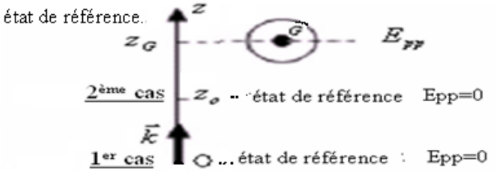
\includegraphics[width=0.5\textwidth]{./img/img00.png}
\end{wrapfigure}
$E_{pp}$: énergie potentielle de pesanteur en (J).
\\g : l'intensité de pesanteur en (N/kg).
\\C: constante qui se détermine à partir de l'état de référence.
\\z: l'altitude du centre de gravité du corps en (m).



Par convention $E_{pp}$=0 pour z=0 (normalement au sol) donc Cte=0 : $E_{pp} = m. g. z$
\em{
    \\- Il est possible de choisir le niveau de référence pour l'énergie potentielle (Epp=0) à une altitude quelconque}
\\\em{- L'énergie potentielle de pesanteur d'un solide dépend de son altitude z, c'est à dire de sa position par rapport à la Terre.
}

\begin{itemize}

    \item \textbf{1er Cas : si l'état de référence est Epp = 0 lorsque z = 0 :}
        \\{
            $E_{pp} = m.g.z + C$ donc $ 0 = m.g.0 + C$ alors $C = 0$dans ce cas $E_{pp}=m.g.z$ 
        }

    \item \textbf{2ème Cas : si l'état de référence est Epp = 0 lorsque z = $z_0$ :}
\\{
$E_{pp} = m.g.z + C$ donc $ 0 = m.g.z_0 + C$ alors $C = mgz_0$dans ce cas $E_{pp}=m.g.(z-z_0)$ 
        }
\end{itemize}
Remarque : 
\\-l'énergie potentielle est une valeur algébrique.
\\-La valeur de l'énergie potentielle de pesanteur d'un corps dépend du choix de l'état de référence


\section{Variation de potentielle de pesanteur : }

Lorsqu'un corps se déplace de la position G1 à la position G2 , la variation de son énergie de potentielle : $$\Delta E_{pp} = E_{pp2} - E_{pp1} = m.g.(z_2 - z_1)$$
Or nous savons que le travail du poids d'un corps durant le déplacement de G1 à G2 : 
$$W(\vec{P})_{G_1\rightarrow G_2} = m.g.(z_1 - z_2)$$

D'aprèes(1) et 2 on déduit que : $$\Delta E_{pp} = -  W(\vec{P})_{G_1 \rightarrow G_2}$$

pour : $\Delta E_{pp} > 0$ ,$(z_2 - z_1) > 0$ le corps gagne de l’énergie potentielle au cours de sa montée

pour : $\Delta E_{pp} < 0$ ,$(z_2 - z_1) < 0$ le corps perd de l’énergie potentielle au cours de sa descente

\section{Energie mécanique : }

\subsection{Définition : }
L'énergie mécanique d'un corps solide à un instant donné est la somme de son énergie cinétique et son énergie potentielle de pesanteur à cet instant :
$$E_m = E_c + E_{pp}$$
\\EM : énergie mécanique en (J)
\\Ec : énergie cinétique en (J)
\\Epp : énergie potentielle de pesanteur en (J)

\subsection{Conservation de l'énergie mécanique du solide : }
\subsubsection{Cas d'un corps en chute libre : }

\begin{wrapfigure}[10]{r}{0.2\textwidth}
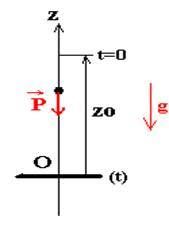
\includegraphics[width=0.2\textwidth]{./img/img01.jpeg}
\end{wrapfigure}


On considère un corps solide de masse m en chute libre sous l'action de son poids.
\\En appliquant le théorème de l'énergie cinétique sur le corps entre les positions G1et G2:
\\$\Delta E_{c} = \sum W_{G_1 \rightarrow G_2}(\vec{F})$
le corps en chute librer est soumis uniquement a l'action de son poids , donc  \\$\Delta E_{c} = W_{G_1 \rightarrow G_2}(\vec{P})$  donc $$\Delta {E_c}_{G_1 \rightarrow G_2} =m.g(z_1 - z_2)   (1)$$  (1) 
l'énergie potentielle de pesanteur du corps dans la position G1 : $E_{pp1} = m.g.z_1 + C$
\\l'énergie potentielle de pesanteur du corps dans la position G2 : $E_{pp2} = m.g.z_2 + C$
\\Donc la variation de l’énergie potentielle du corps entre G1 et G2 est : \\$\Delta E_{pp} = E_{pp_2} - E{pp_1} = m.g.z_2 + C - (m.g.z_1 + C)$
$$\Delta E_{pp} = m.g.(z_2 - z_1) \;\;\;\; (2)$$
d'après (1) et (2) on a :
$$\Delta {E_c}{G_1 \ rightarrow G_2} =\Delta {E_{pp}}{G_1 \ rightarrow G_2} $$
$$E_{c_2} - E_{c_1} = -(E_{pp2} - E_{pp1})$$
$$E_{c_2} + E_{pp2} = E_{c_1}  + E_{pp1})$$
$$E_{m2} = E_{m1}$$
Donc il y'a conservation de l'énergie mécanique du corps entre les positions G1 et G2.

\subsubsection{Cas de glissement d'un corps solide sans frottement sur un plan incliné : }


\begin{wrapfigure}[10]{r}{0.2\textwidth}
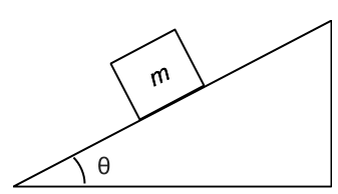
\includegraphics[width=0.2\textwidth]{./img/img02.png}
\end{wrapfigure}

On considère un corps solide en état de glissement sans frottement sur un plan incliné comme l'indique la figure suivante: 
Le corps est soumis à l'action de deux forces :
\\$\vec{P} : son poids$
\\$\vec{R}$ : la réaction du plan incliné.
\\En appliquant le théorème de l'énergie cinétique sur le corps entre les positions A et B:
$$\Delta {E_c}_{A \rightarrow B} =\sum {W(\vec{F})}_{A \rightarrow B}$$

$$\Delta {E_c}_{A \rightarrow B} = {W(\vec{P})}_{A \rightarrow B} + {W(\vec{R})}_{A \rightarrow B} \; \;\;\; avec \; \; \; {W(\vec{R})}_{A \rightarrow B} = 0$$
$$alors \;\;  \Delta {E_c}_{A \rightarrow B} = {W(\vec{P})}_{A \rightarrow B} or \Delta {E_{p}}_{A \rightarrow B} = -{W(\vec{P})}_{A \rightarrow B} $$
$$donc \;\;\; \Delta {E_{c}}_{A \rightarrow B} = - \Delta {E_p}_{A \rightarrow B} $$
$${E_c}_{(B)} - {E_c}_{(A)} = {E_p}_{(B)} - {E_p}_{(A)}$$
$${E_c}_{(B)} + {E_p}_{(B)} = {E_c}_{(A)} + {E_p}_{(A)}$$

$${E_m}_{(B)} = {E_m}_{(A)} $$
Donc il y'a conservation de l'énergie mécanique du corps entre A et B.
On dit que le poids est une force conservative , car malgré que le poids travail au cours du mouvement il y'a conservation de l'énergie mécanique.

\section{Non conservation de l'énergie mécanique du solide : (Sc. Math) }

\begin{wrapfigure}[4]{r}{0.2\textwidth}
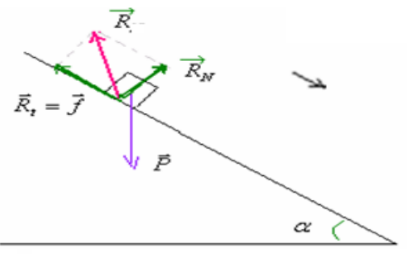
\includegraphics[width=0.2\textwidth]{./img/img03.png}
\end{wrapfigure}



Quand le poids est la seule force à travailler (comme dans le
mouvement de chute libre), on peut écrire, en appliquant le théorème
de l'énergie cinétique entre deux instants t1 et t2
quelconques.

Le mouvement d'un corps solide avec frottement sur un plan incliné : 

Le corps est soumis à l'action de deux forces :
\\$\vec{P} : son poids$
\\$\vec{R}$ : la réaction du plan incliné.
\\En appliquant le théorème de l'énergie cinétique sur le corps entre les positions A et B:
$$\Delta {E_c}_{A \rightarrow B} =\sum {W(\vec{F})}_{A \rightarrow B}$$

$$\Delta {E_c}_{A \rightarrow B} = {W(\vec{P})}_{A \rightarrow B} + {W(\vec{R})}_{A \rightarrow B} \; \;\;\; avec \; \; \; {W(\vec{R})}_{A \rightarrow B} \ne 0$$

$$
 \left \{
   \begin{array}{r c l}
       {W(\vec{R})}_{A \rightarrow B}  & = & W(\vec{R}_N) + W(\vec{f}) = W(\vec{f}) \\
       W(\vec{P}) & = & -\Delta E_p
   \end{array}
   \right .
$$
donc 
$$ \Delta {E_c}_{A \rightarrow B} = -\Delta E_p  + W(\vec{f})  $$

$$ \Delta {E_c}_{A \rightarrow B}  + \Delta E_p  =  W(\vec{f})  $$


$$ \Delta {E_m}_{A \rightarrow B} = W(\vec{f})  $$
Interprétation: Les forces de frottements ne sont pas conservatives car à cause de leur travail l'énergie mécanique du système diminue, cette
diminution est due à une perte d'une partie de l'énergie mécanique par frottement sous forme d'énergie calorifique (chaleur) .
$$ \Delta {E_m}_{A \rightarrow B} = W(\vec{f}) = -Q$$

\end{document}

